\documentclass[a4paper,12pt]{article}
\usepackage{cmap}
\usepackage{dsfont}
\usepackage[T2A]{fontenc}
\usepackage[utf8]{inputenc}
\usepackage[english,russian]{babel}
\usepackage{amsmath,amsfonts,amssymb,amsthm,mathtools,mathtext}
\usepackage[left=2.5cm,right=2.5cm,top=2cm,bottom=2cm]{geometry}
\usepackage{graphicx}
\usepackage[colorlinks,linkcolor=blue]{hyperref}
\usepackage{physics}
\usepackage{esvect}
\usepackage{icomma}
\usepackage{indentfirst}
\usepackage[labelsep=period,justification=centering]{caption}
\setlength{\parindent}{1.25cm}
\title{Введение в машинное обучение}
\author{Гладышев Денис}
\date{ноябрь 2026}

\begin{document}

\maketitle
Перед началом главных определений стоит отметить, что не все задачи следует решать с помощью методов машинного обучения. Если алгоритм прост в плане математической и вычислительной сложности, например, поиск точек экстремума функции $f(x)=x^2-2x+5$, то лучше решить задачу классическими методами.

Основные же задачи, рассматриваемые в данном введении - это следующий класс задач:
\begin{enumerate}
    \item Задачи \textit{классификации} - подаваемые данные необходимо отнести к какому-то классу, например, распознать на фотографии кошку или собаку. 
    \item Задачи \textit{регрессии} - прогноз в виде вещественных чисел на основе входных данных, например, прогноз поведения функции по некоторым измеренным эмпирическим данным. 
    \item Задачи \textit{ранжирования} - упорядочивание по некоторому критерию входных данных, например, модель поисковой системы.
\end{enumerate}
\section{Введение в машинное обучение.}
\subsection{Обучающая выборка.}
\noindent\textbf{Определение.1.1.1.}Пусть нам подаются некоторые исходные данные, прямые результаты измерений, представляемые в виде некоторых чисел. Все эти результаты измерений будет удобно представлять в виде следующих векторов:
\begin{equation*}
    x_i = 
    \begin{bmatrix}
    x_{i1}\\
    x_{i2}\\
    ...\\
    x_{in}
    \end{bmatrix}
    =
    \begin{bmatrix}
        x_{i1} & x_{i2} & ... & x_{in}
    \end{bmatrix}
    ^T
\end{equation*}
где $x_i$ - результаты измерений некоторого $i$-го объекта. Например, нам дано N человек, и у каждого из них мы измерили рост и вес. Тогда результат измерений $k$-го человека можно записать как вектор $x_k=[x_{k1} \  x_{k2}]^T$.

Все эти наборы результатов, для всех объектов, можно записать в одну единую матрицу $X$, \textit{матрицу признаков}, представленную ниже.
\begin{equation*}
    X = 
    \begin{bmatrix}
        x_1\\
        x_2\\
        ...\\
        x_l
    \end{bmatrix}
    =
    \begin{bmatrix}
        x_{11} & x_{12} & ... & x_{1n} \\
        x_{21} & x_{22} & ... & x_{2n} \\
        . & . & . & .\\
        x_{l1} & x_{l2} & ... & x_{ln}
    \end{bmatrix}
\end{equation*}
где $l$ - число объектов, которые мы измеряем, $n$ - количество признаков, например, в случае $N$ людей, у которых мы измерили рост и вес, получится матрица размером $N \times2$.

\newpage
\noindent\textbf{Определение.1.1.2.}Для полноты картины нам также необходимо определить выходные данные, \textit{целевые значения}, представляемые в виде вектора $Y$, определенного ниже.
\begin{equation*}
    Y =
    \begin{bmatrix}
        y_1\\
        y_2\\
        ...\\
        y_l
    \end{bmatrix}
    =
    \begin{bmatrix}
        y_1 & y_2 & ... & y_l
    \end{bmatrix}
    ^T
\end{equation*}

\noindent\textbf{Замечание.}Обратите внимание, что для $l$ объектов, которые мы как-то измеряем, вектор целевых значений имеет $l$ компонент.\\

\noindentЧто же это за вектор такой? В зависимости от задачи, он может принимать разные значения. Посмотрим примеры:
\begin{enumerate}
    \item В задачах \textit{бинарной классификации} $y_i\in\{1,-1\}$.
    \item В задачах \textit{M-классовой классификации с непересекающимися классами} $y_i\in\{1,2,...,M\}$.
    \item В задачах \textit{одномерной регрессии} $y_i\in\mathds{R}$.
    \item В задачах \textit{$m$-мерной регрессии} $y_i\in\mathds{R}^m$.
\end{enumerate}
и так далее...\\

\noindent\textbf{Определение.1.1.3.}\textit{Обучающей выборкой} или \textit{размеченными данными} называется совокупность входных измерений и соответствующих целевых значений, то есть следующий набор пар:
\begin{equation*}
    X^l = \{(x_i, y_i)_{i=1}^l\}
\end{equation*}\\

\noindent\textbf{Замечание.}Иногда входные данные измерений могут быть слишком тяжелыми для работы с ними, например, если нам дают вектор признаков $x$ для звукового файла, в который мы записываем амплитуды, то этот вектор получится слишком большой и работать с ним напрямую очень тяжело. Чтобы упростить себе работу, мы используем так называемые \textit{вторичные признаки}. Смысл в том, что мы строим более информативные признаки для нашего объекта, используя некоторые функциональные преобразования $f_1, ..., f_k$, получая новый вектор признаков для объекта $x$ - $[f_1(x), ..., f_k(x)]^T$. Тогда наша матрица признаков $X$ для $l$ объектов с $n$ признаками преобразуется в матрицу $F$, имеющую следующий вид.
\begin{equation*}
    F = [f_j(x_i)]_{i=1}^l =
    \begin{bmatrix}
        f_1(x_1) & f_2(x_1) & ... & f_k(x_1) \\
        f_1(x_2) & f_2(x_2) & ... & f_k(x_2) \\
        . & . & . & .\\
        f_1(x_l) & f_2(x_l) & ... & f_k(x_l)
    \end{bmatrix},\quad j=1,...,k
\end{equation*}

\newpage
\subsection{Постановка задачи машинного обучения.}
\noindentПусть нам даны выборка $X^l = \{(x_i,y_i)_{i=1}^l\}$ и признаковое пространство $F = [f_j(x_i)]_{l\times n}$. Предположим, что на вход некоторой модели(алгоритма) подается набор признаков $f_j(x_i)$ некоторого объекта $x_i$ и на выходе должно формироваться некоторое целевое значение $y_i=y(x_i)$, но модель этого значения не знает и выдает свое $a_i=a(x_i)$. Тогда наша задача заключается в том, чтобы подобрать такую модель, что выдаваемые значения $a_i$ в среднем мало отличались от $y_i$.\\

\noindent\textbf{Определение.1.2.1.}Нетрудно понять, что модель мы будем подбирать по обучающей выборке, потому что для $x_i$ мы уже знаем выходные целевые значения $y_i$. Благодаря этому мы можем решить поставленную задачу. Такой подход называется \textit{обучением} и в результате него формируется \textit{решающая функция} $a_i=a(x_i)$. Тогда наша модель будет обладать \textit{обобщающей способностью}, то есть она сможет работать не только в пределах обучающей выборки, но и на всем множестве всех возможных входных данных того же типа.\\

\noindentПо сути это и есть \textbf{общая постановка задачи машинного обучения}. Но как же тогда искать функцию $a(x)$?

\subsection{Принцип параметрической оптимизации.}
Один из самых простейших подходов нахождения решающей функции $a(x)$ - это представить ее в следующем виде:
\begin{equation*}
    a(x)=g(x, \theta)
\end{equation*}
где функция $g$ зависит от набора параметров $\theta = [\theta_1 \ \theta_2 \ ...\ \theta_n]^T$. Тогда наша задача сводится к поиску этих параметров. Искать мы их будем, понятное дело, с помощью обучающей выборки, так как другого нам не дано.\\

\noindent\textbf{Пример: линейная регрессия}.

\noindentПусть нам дана явная зависимость между входами и выходами, например, линейная, и мы формируем наши целевые значения следующим образом:
\begin{equation*}
    y_i = kx_i+b+\mathcal{E}_i, \quad \mathcal{E}_i \sim \mathcal{N}(0, \sigma^2)\text{ - гауссовский шум}\label{eq1}
\end{equation*}
Тогда нашу функцию $g$ можно построить следующим образом: $g(x,k,b)=kx+b$ (шум не учитываем). Если построить множество точек $(x_i, y_i)$ и функцию $g$, то мы увидим, что точки разбросаны вблизи прямой. Это и есть наше приближение, и в будущем, если будут подаваться еще какие-то данные и по ним строиться целевые значения, то точки также будут находиться вблизи прямой. Получаем, что в нашей задаче $\theta=[k \ b]^T$\\

\noindent\textbf{Определение.1.3.1.}Пусть, как и раньше, $a(x)=g(x,\theta)$. Мы хотим найти значения параметров $\theta$ на множестве входов и выходов обучающей выборки $X\times Y$, то есть подобрать эти параметры так, чтобы уменьшить ошибку между заданным входом и выходом модели: $a(x)-y(x)$ $\forall x$, однако эта ошибка не очень удобна в качестве оптимизируемой величины, так как в нуле у нее нет точки экстремума. Поэтому для наших целей мы будем использовать специальные функции, получившие названия \textit{функции потерь}.
\newpage
\noindentБывают разные функции потерь, например,
\begin{align*}
    & \hspace{-7cm}L(a, x) = |a(x)-y(x)| \text{ - \textit{абсолютная ошибка}}\\
    & \hspace{-7cm}L(a, x) = (a(x)-y(x))^2 \text{ - \textit{квадратичная ошибка}}
\end{align*}
однако все они удовлетворяют одному свойству: чем больше ошибка $a(x)-y(x)$, тем больше значение функции потерь и наоборот.\\

\noindentНетрудно увидеть, что функция потерь является случайной величиной, которая зависит от алгоритма $a$ и значения $x$, то есть при разных $x$ мы получаем разные значения функции, поэтому необходимо, чтобы на всем обучающем множестве в среднем ошибка была бы минимальна. Из этих рассуждений мы приходим к следующему определению.\\

\noindent\textbf{Определение.1.3.2.}\textit{Средним эмпирическим риском} называется функция $Q$, определенная как
\begin{equation*}
    Q(a, X^l)=\frac{1}{l} \sum_{i=1}^lL(a, x_i), 
\end{equation*}
где $X^l = \{(x_i,y_i)_{i=1}^l\}$ - обучающее множество. Поэтому нам необходимо выбрать такие параметры $\theta$, чтобы для полученной модели $a(x)$ ее средний эмпирический риск был наименьшим среди всех возможных. Тогда и мы получим нужный алгоритм.\\

\noindent\textbf{Пример:}
Вспомним линейную регрессию \ref{eq1} и в качестве функции потерь выберем квадратичную. Тогда наша функция среднего эмпирического риска примет следующий вид:
\begin{equation*}
    Q(a, X^l)=\frac{1}{l}\sum_{i=1}^l(a(x_i)-y(x_i))^2 = \frac{1}{l}\sum_{i=1}^l(kx_i+b-y(x_i))^2
\end{equation*}
Тогда, чтобы минимизировать нашу функцию, то есть найти параметры $k$ и $b$, достаточно решить следующую систему:
\begin{equation*}
\begin{cases}
 \frac{\partial Q(a, X^l)}{\partial k} = \sum\limits_{i=1}^l(kx_i+b-y(x_i))\cdot x_i = 0\\
 \frac{\partial Q(a, X^l)}{\partial b} = \sum\limits_{i=1}^l(kx_i+b-y(x_i))=0
\end{cases}
\end{equation*}
Такой подход называется \textit{методом наименьших квадратов}. Подробнее о нем мы поговорим в отдельной главе.\\

\noindentВсе вышесказанное можно математически записать так:

\noindentЕсли $a(x)=g(x,\theta)$ - параметрическая модель, то \textit{обученной моделью} называется модель $a=\mu(X^l)$, где
\begin{equation*}
    \mu(X^l)=arg\min\limits_\theta Q(a,X^l)
\end{equation*}

\subsection{Линейная модель.}
\noindentВспомним пример \ref{eq1}. Как мы помним, оптимальной моделью является следующая функция: $a(x)=\hat{k}x+\hat{b}$ (параметры отличны от $k$ и $b$, потому что в общем случае они подбираются по обучающей выборке, поэтому могут содержать некоторые погрешности). Однако, эту же самую модель можно записать в виде $a(x)=\theta_1\cdot f_1(x)+\theta_2\cdot f_2(x)$, где $f_j(x)$ - признаки, $\theta_j$ - некоторые параметры ($j=1,2$). Мы получаем, своего рода, общий вид линейной модели, и при $\theta_1=\hat{k}, \theta_2=\hat{b}$ и $f_1(x)=x, f_2(x)=1$ мы получим нашу оптимальную модель $a(x)$. Обобщим это на случай $n$ разных признаков, и получим \textit{общий вид линейной модели}
\begin{equation*}
    a(x)=\sum\limits_{i=1}^n\theta_i\cdot f_i(x),
\end{equation*}
где $\theta=[\theta_1 \ \theta_2 \ ... \ \theta_n]^T$. Заметим, что в координатах ($f_1(x),f_2(x),...,f_n(x)$) мы получаем уравнение \textit{гиперплоскости}, а наш вектор $\theta$ задает ориентацию этой плоскости (вектор нормали к плоскости).\\

\noindentРазберем следующий \textbf{пример} задачи линейной регрессии:

\noindentПредположим, что мы будем строить наше множество целевых значений по следующей формуле:
\begin{equation*}
    y(x)=\sin(x)+0.3x+\mathcal{E}(x), \ x\in[0,5]
\end{equation*}

\noindentПолучим следующее множество точек (для конкретного шума $\mathcal{ E}$):\\

\begin{figure}[htbp]
    \centering
    \includegraphics[width=0.8\textwidth]{plot.pdf}
    \caption{}
    \label{fig:points}
\end{figure}

\noindentТо есть у нас всего 1 признак $x$, по которому строится целевое значение $y(x)$. Казалось бы, линейная модель будет иметь вид $a(x)=\theta_1x$ для одного параметра $\theta_1$, однако, если построить эту прямую, то видно, что она не аппроксимирует наше множество точек, потому что между $x$ и $y(x)$ более сложная зависимость, чем линейная. Поэтому мы пойдем на некоторую хитрость: расширим наше признаковое пространство так, чтобы мы оставались в рамках линейной модели. Сделаем мы это так: положим $f_0(x)=1, f_1(x)=x, f_2(x)=x^2,...,f_n(x)=x^n$. Важно, чтобы полученное расширенно множество признаков было \textbf{линейно независимым}, иначе тогда один из признаков выражается через другие, а значит, никакой новой дополнительной информации он не несет и мы сделали лишнее действие. После нашего расширения мы получим новую линейную модель, имеющую вид
\begin{equation*}
    a(x)=1\cdot \theta_1 + x \cdot\theta_2 + x^2\cdot\theta_3 + ...+x^n\cdot\theta_{n+1},
\end{equation*}
где $\theta=[\theta_1 \ \theta_2 \ ... \ \theta_n \ \theta_{n+1}]^T$. В частности, этот набор параметров можно найти по методу наименьших квадратов. Своего рода, мы построили \textit{многочлен Тейлора}, который хорошо приближает нашу функцию в нуле. Однако, приближение такими полиномами не всегда решает задачу. Возьмем функцию $y(x)$ и приближающий ее полином $a(x)$ следующим образом:
\begin{equation*}
    y(x)=\frac{1}{1+10x^2}, \ \ \ a(x)=\sum\limits_{i=1}^{54}\theta_i\cdot x^i,
\end{equation*}
где $x\in[0,10]$, при этом будем вычислять коэффициенты полинома лишь по половине точек, взятых через отсчет. По другой половине модель будет строить прогноз. Получим следующее:

\begin{figure}[htbp]
    \centering
    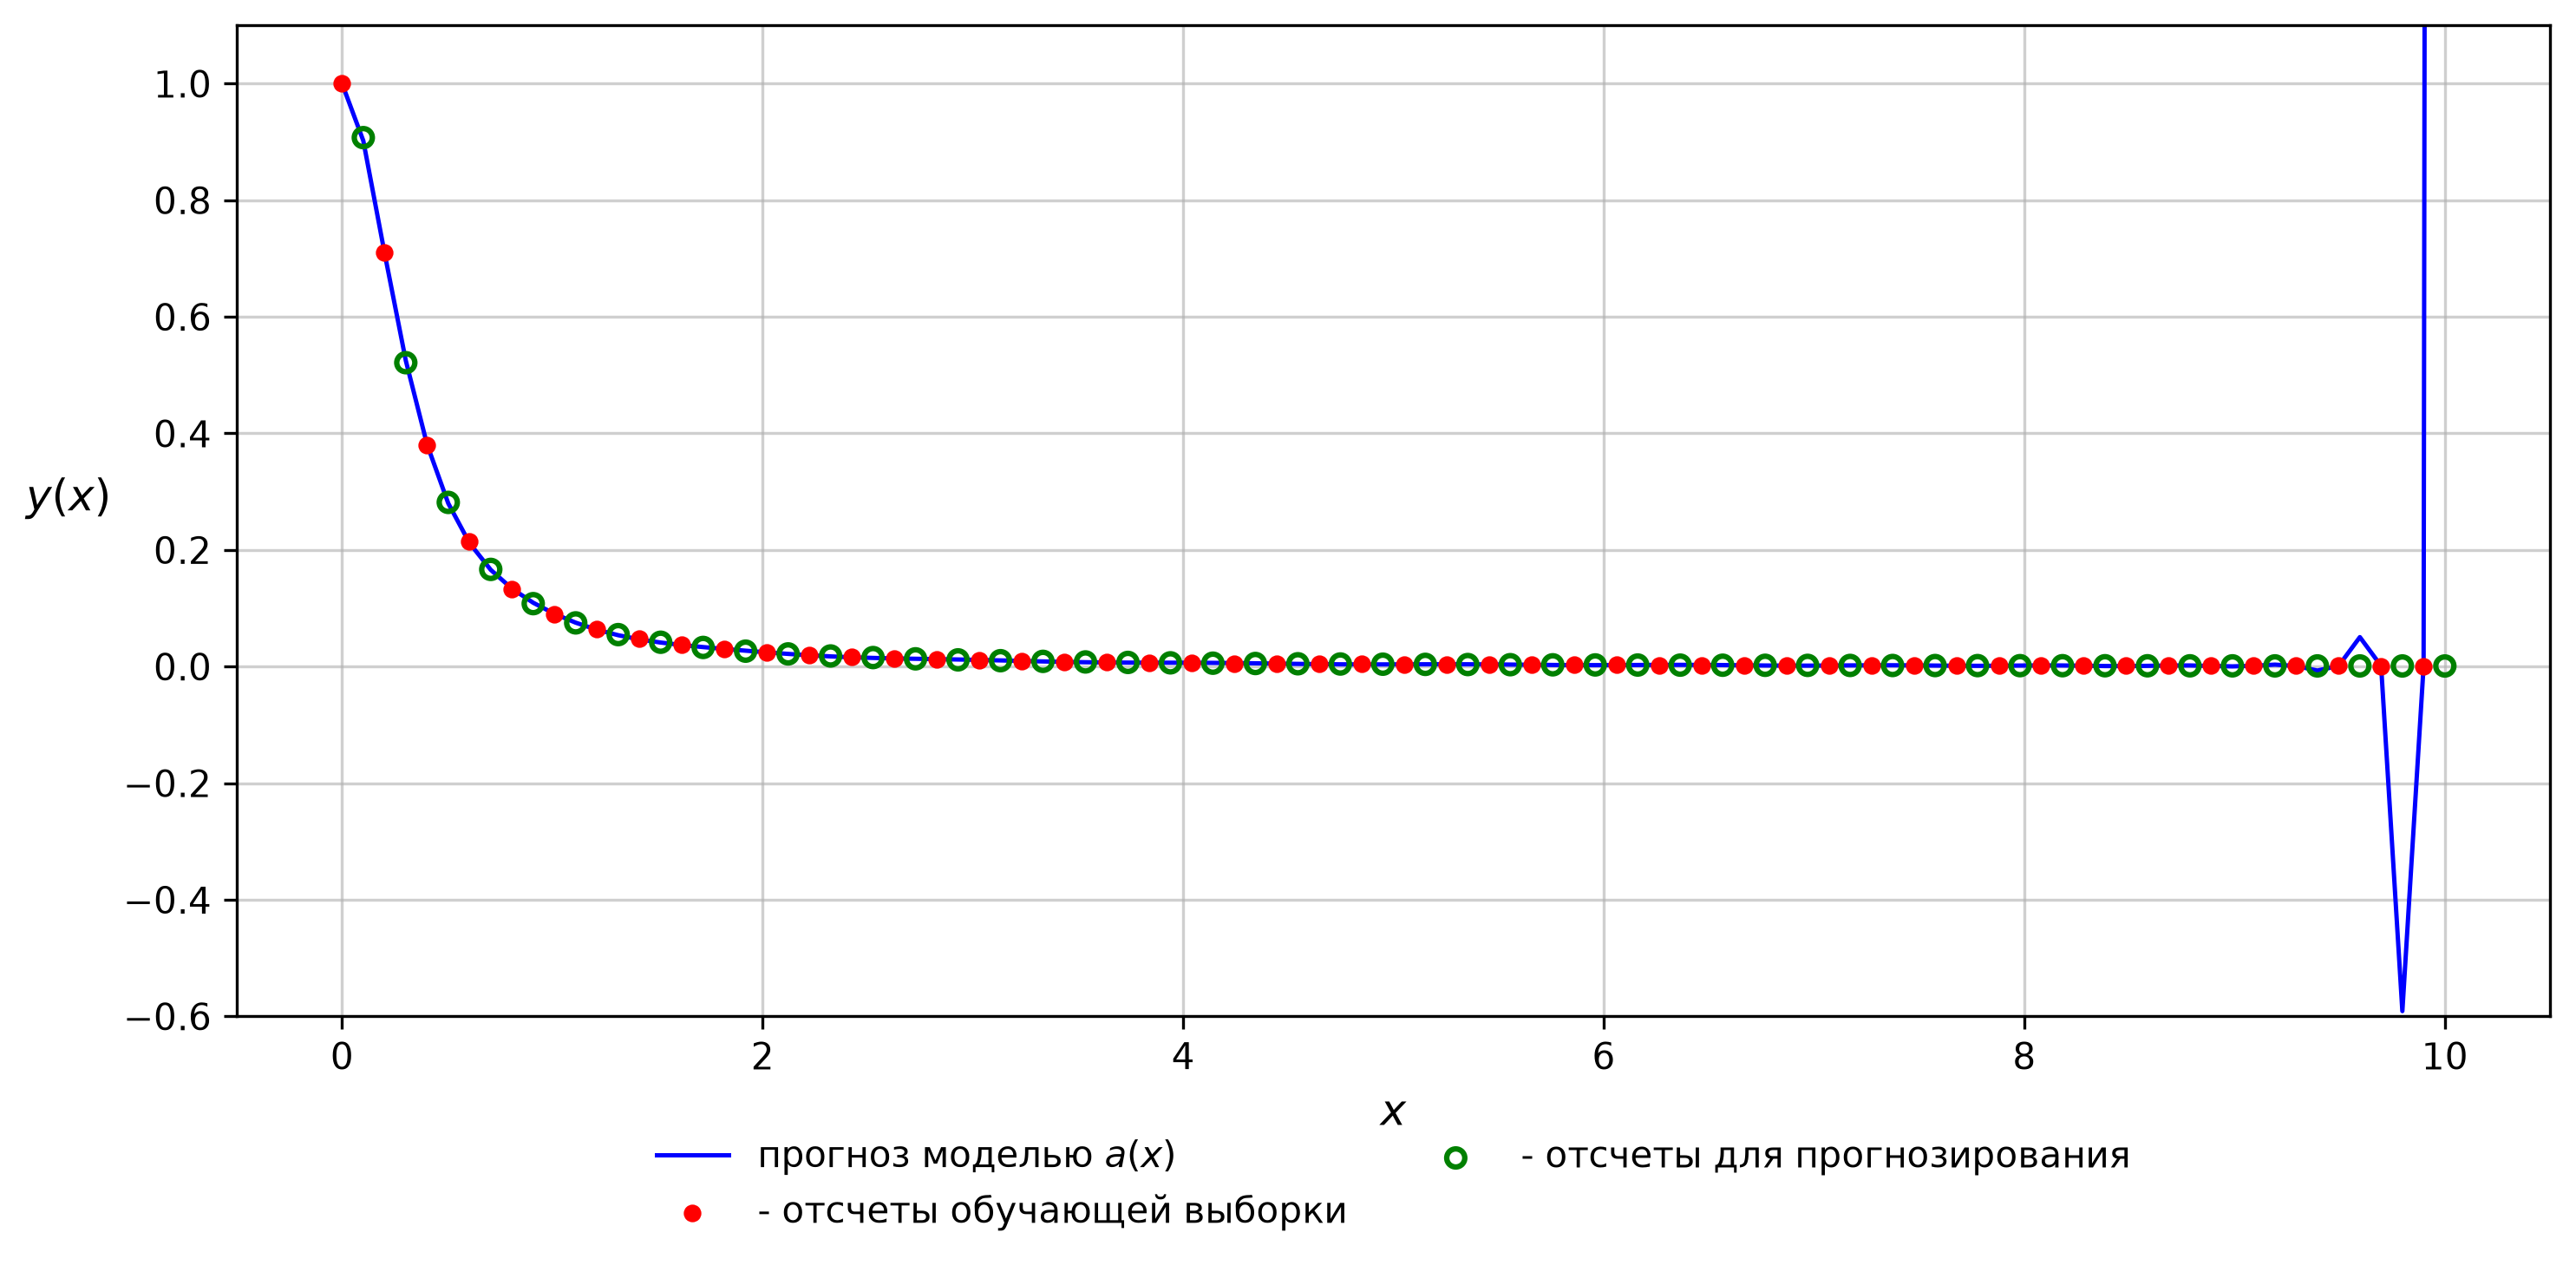
\includegraphics[width=0.9\textwidth]{polynomial_overfitting.png}
    \caption{}
    \label{fig:overfitting}
\end{figure}

\noindentВидим, что при больших $x$ полином ведет себя непредсказуемо. Это означает, что модель будет плохо строить прогнозы в новых, неизвестных ей точках. Но для полиномов маленькой степени таких проблем обычно нет. Здесь мы приходим к новому понятию, названному \textit{переобучением}.\\

\noindent\textbf{Определение.1.4.1.}\textit{Переобучение} - несоответствие найденной модели $a(x)$ закону изменения данных, часть которых была представлена в обучающей выборке. При этом данные самой обучающей выборки описываются хорошо. То есть модель не обладает достаточной обобщающей способностью.\\

\noindent\textbf{Замечание.}Здесь становится понятно, что нам не только важно построить функцию по эмпирическим зависимостям, а понять закон, модель этих зависимостей. В этом будет заключаться главная задача машинного обучения. Однако, любая модель будет обладать той или иной степенью переобучения. Избавиться от него невозможно, поэтому нашей единственным выходом останется минимизировать данный эффект и, как следствие, увеличить обобщающую способность модели.

\newpage
\subsection{Оценка переобучения модели.}

\subsubsection{Оценка по отложенной выборке.}
\noindentМетод заключается в том, что мы делим размеченные данные на 2 части: \textit{обучающую} и \textit{отложенную}(hold-out). Заметим, что деление происходит случайно и как правило соотношение обучающей выборки к отложенной составляет $70\%$ к $30\%$.

\noindentДалее для найденной модели строятся качество работы для обучающей выборки - $Q_1(a, X^l)$, и для отложенной выборки - $Q_2(a, X^t)$. Если величины оказываются близкими, то модель считается \textit{приемлемой}, а иначе, когда $Q_2$ значительно больше $Q_1$, переобученной.\\

\noindent\textbf{Замечание.}Недостаток такого метода заключается в способе разбиения на обучающую и отложенную выборки, ведь случайно может оказаться так, что по данному разбиению модель будет приемлемой, но на практике качество будет заметно ниже.

\subsubsection{Скользящий контроль.}
\noindentИдея следующая: будем из нашей обучающей выборке поочередно убирать один вектор наблюдения и обучаться на оставшемся наборе размеченных данных. Так мы получим некоторую модель $a_1(x)$. Далее возвращаем этот вектор в исходную выборку и убираем следующий. Получим модель $a_2(x)$. И так далее...
В итоге, мы получим набор различных моделей $a_1(x)$, $a_2(x)$, ..., $a_l(x)$, где $l$ - число объектов наблюдения в исходной обучающей выборке.

\noindentПосле данной процедуры мы формируем новую модель на основе полученных, которая обладала бы наилучшей обобщающей способностью: $a(x) = F(a_1,a_2, ..., a_l)$.\\

\noindent\textbf{Замечание.}Хоть данный способ и решает проблему прошлого, однако он вычислительно сложный, ведь нам надо $l$ раз обучаться и строить модель, а потом еще и как-то придумать модель $F(a_1,..., a_l)$, решающую нашу задачу.

\subsubsection{Кросс-валидация.}
\noindentПо сути, тоже самое, что и скользящий контроль, однако мы уже разбиваем обучающую выборку на какие-то группы векторов (зачастую на $k-1$ равных по количеству объектов групп, причем в $k$ их может быть меньше) и поочередно их выкидываем, обучаясь по оставшейся выборке. Получая модель $a_j(x)$, мы возвращаем группу на место в исходную выборку. В итоге мы получим набор моделей $a_1(x)$, $a_2(x)$, ..., $a_k(x)$, по которым построим модель $a(x)=F(a_1,a_2,...,a_k)$, решающую нашу задачу.\\

\noindentК сожалению, нет единого способа построить наилучшую модель, мы сами должны понять, как лучше скомбинировать полученные модели.

\subsection{Уравнение гиперплоскости в задачах бинарной классификации.}
\noindentНачнем изучение довольно интересной темы машинного обучения - \textit{классификации входных данных}. Данные алгоритмы применяются во многих областях нашей жизни: это и камеры с распознаванием лица, проверка отпечатка пальца в телефоне, доступ к каким-либо данным по голосу и прочее. Во всех этих алгоритмах лежит один простой принцип, который мы изучим в этом разделе, - \textit{построение разделяющей гиперплоскости} в определенном признаковом пространстве.\\

\noindentДля простоты мы рассмотрим задачу двухклассовой классификации точек на плоскости. То есть каждый объект наблюдения представляется в виде вектора с двумя координатами: $x_i = [x_{i1} \ x_{i2}]^T, \ i=1,2,..$. Целевые значения определим следующим образом:
\begin{equation*}
    y_i=
    \begin{cases}
        +1, x_i\in C_1 \\
        -1, x_i\in C_2
    \end{cases}
    , \ \text{где }C_1, C_2 \text{ - какие-то классы данных.} 
\end{equation*}

\noindentГрафически, распределение двух классов можно представить, например, так: 
\begin{figure}[h]
    \centering
    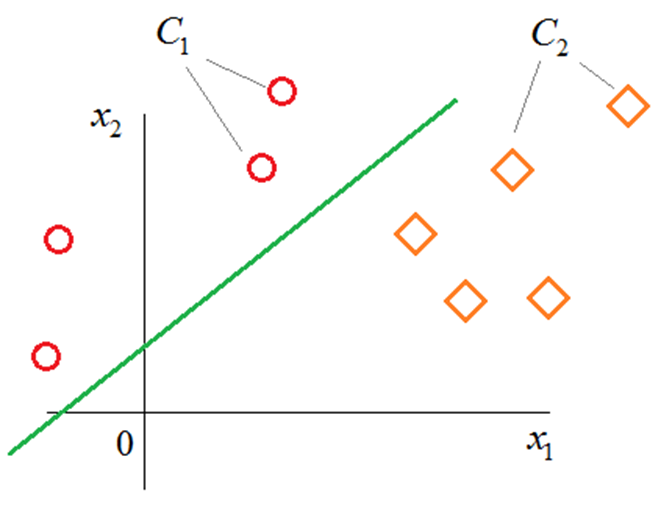
\includegraphics[width=0.6\textwidth]{image.png}
    \caption{}
    \label{fig:myimage}
\end{figure}

\noindentВ качестве модели в этой задаче выступает уравнение разделяющей зеленой прямой: $a(x)=kx+b$. Как описать множество точек, лежащих на данной прямой? В общем, это точки, связанные соотношением $x_2=a(x_1)$, то есть
\begin{align*}
    x_2 &= kx_1+b\\
    x_2 - &kx_1 - b = 0
\end{align*}

\noindentВ общем виде это можно записать так:
\begin{equation*}
    w_1x_1+w_2x_2-w_0=0
\end{equation*}
Например, для $\{w_1,w_2,w_0\}=\{-k,1,b\}$ получим нашу прямую $x_2=kx_1+b$. Если выделить два вектора: $w=[w_1 \ w_2]^T, \ x=[x_1 \ x_2]^T$, то общий вид можно переписать так:
\begin{gather*}
    \langle w, x \rangle - w_0 = 0, \\
    \text{где } \langle w, x \rangle = w^T x = w_1 x_1 + w_2 x_2
    \text{ --- \textit{скалярное произведение} векторов } w, x.
\end{gather*}
Для удобства положим $w_0=0$. Он определяет сдвиг прямой, поэтому предположим, что прямая проходит через начало координат. Возьмем в качестве вектора $w$ вектор $w=[-1 \ 1]^T$. Тогда мы получим уравнение прямой $x_2=x_1$, то есть наша модель имеет вид: $a(x)=x$. Заметим, что вектор $w$ будет ортогонален этой прямой. Вообще говоря, это \textit{вектор нормали} к нашей прямой. Заметим, что для любой прямой вида $\langle w,x\rangle-w_0=0$ вектор $w$ будет ей ортогонален.\\

\newpage

\begin{figure}[h]
    \centering
    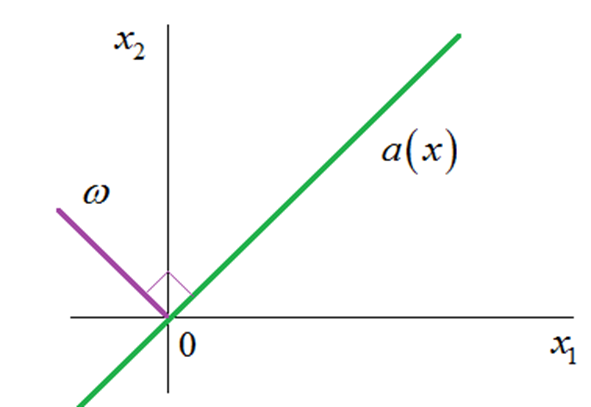
\includegraphics[width=0.6\textwidth]{image (1).png}
    \caption{Прямая $x_2=x_1$. $w$ - нормаль к прямой.}
    \label{fig:myimage}
\end{figure}

\noindentДавайте в уравнении $\langle w, x\rangle - w_0=0$ положим $w=[w_0 \ w_1 \ w_2]^T$, а $x=[-1 \ x_1 \ x_2]^T$. Тогда мы получим уравнение плоскости в трехмерном пространстве. Гиперплоскость будет вращаться относительно нуля, а вектор $w$ будет по-прежнему ортогонален плоскости. То есть, как видите, для вектора размерности $n$ мы всегда можем добавить еще одно измерение, чтобы создать гиперплоскость, проходящую через ноль.

\begin{figure}[h]
    \centering
    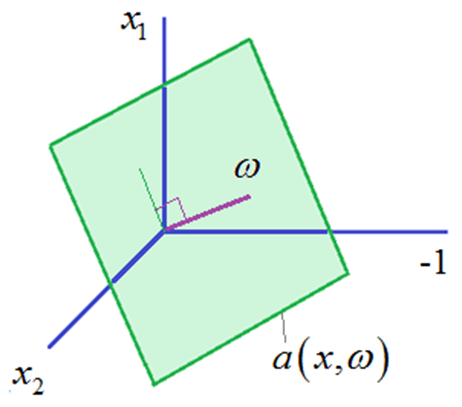
\includegraphics[width=0.6\textwidth]{image (2).png}
    \caption{Плоскость $\langle x, w\rangle=0$.}
    \label{fig:myimage}
\end{figure}

\noindentДавайте рассмотрим модель $a(x,w)=\langle x, w\rangle$, задающую прямую $a(x,w)=0$ на плоскости. Как, используя эту модель, отделять объекты одного класса от другого? Смотрите, если наша модель построена правильно, и прямая действительно делит образы точек на плоскости на два класса, то используем следующее наблюдение: точки из класса $C_1$ образуют с вектором $w$ острый угол, а вот точки $C_2$ - тупой. Тогда можем сделать такой вывод:
\begin{equation*}
    \operatorname{sgn}(\langle x, w\rangle)=
    \begin{cases}
        1,\ x\in C_1\\
        -1, x\in C_2
    \end{cases}
\end{equation*}

\newpage
\noindentВ итоге, алгоритм классификации образов с помощью модели $a(x,w)$ можно записать так:
\begin{equation*}
    a(x,w)=\operatorname{sgn}(\langle x,w\rangle)
\end{equation*}
Если же $\langle x, w\rangle=0$, то выдаем отказ в классификации, ведь непонятно, в каком классе лежит точка. Хотя вероятность попадания точки на прямую очень мала.
\end{document}
